\section{Archimedes' Principle and the Law of Flotation}

\begin{multicols}{2}


\section*{Concept of Upthrust}
\textbf{Archimedes' Principle} states that any object partially or totally immersed in a fluid experiences an upthrust equal to the weight of the fluid displaced by the body.
$$ \text{Upthrust} = \text{Weight of displaced fluid}$$
%$$ \text{Weight in air} - \text{Apparent weight in fluid} = \text{Weight of displaced fluid}$$

\subsection{Verifying Archimedes' Principle}

\begin{center}
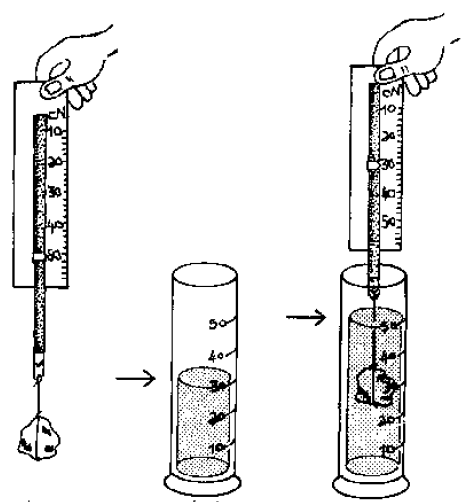
\includegraphics[width=0.4\textwidth]{./img/source/upthrust.png}
\end{center}

\begin{description*}
%\item[Subtopic:]{}
\item[Materials:]{\nameref{sec:spring-balance}, stone, string, \nameref{sec:meascyl}, water, \nameref{sec:eurekacan}, syringe}
%\item[Setup:]{}
\item[Procedure:]{Tie a string around a stone and measure its weight in Newtons using a spring balance. Fill the measuring cylinder partially with water and record the reading. Immerse the stone fully into the water (without touching the bottom) and record the reading on the spring balance, as well as the new water level of the measuring cylinder.}
%\item[Hazards:]{}
\item[Questions:]{What is the change in weight of the stone as read from the spring balance? What is the weight of the displaced water (1 mL = 0.01 N)?}
%\item[Observations:]{}
\item[Theory:]{The change in weight of the stone is known as its \emph{Apparent Loss in Weight}, which is equal to the \emph{Upthrust} exerted on the stone by the water. Archimedes' Principle tells us that this is equal to the weight of the water displaced by the stone.}
%\item[Applications:]{}
\item[Notes:]{A Eureka can and syringe may be used to measure the displaced fluid in place of a measuring cylinder.}
\end{description*}

%==================================================================================================%

\section*{Sinking and Floating}
If the density of an object is less than that of the surrounding fluid, the object will float. If the density is greater than that of the fluid, it will sink.

\textbf{The Law of Flotation} states that a floating body displaces its own weight of the fluid in which it floats.
$$\text{Weight of body} = \text{Weight of displaced fluid}$$


\subsection{Verifying the Law of Flotation}

\begin{center}
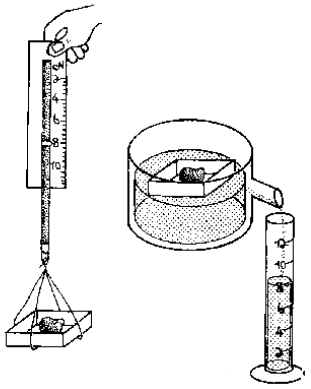
\includegraphics[width=0.4\textwidth]{./img/source/flotation.png}
\end{center}

\begin{description*}
%\item[Subtopic:]{}
\item[Materials:]{\nameref{sec:spring-balance}, matchbox, stone, string, \nameref{sec:eureka-can}, \nameref{sec:meascyl}/syringe}
%\item[Setup:]{}
\item[Procedure:]{Load a matchbox with a small stone so that it still floats in water. Record the weight of the matchbox and stone in Newtons using a spring balance. Fill the Eureka can with water and allow the matchbox to float on it. Collect the overflow in a measuring cylinder or syringe. Calculate the weight of the overflow (1 mL = 0.01 N).}
%\item[Hazards:]{}
\item[Questions:]{How does the weight of the matchbox and stone compare to that of the displaced water?}
\item[Observations:]{The values should be equal, thus verifying the Law of Flotation.}
%\item[Theory:]{}
\item[Applications:]{Submarine, hot air balloon, ships. Design and selection of materials for these vessels are done using the Law of Flotation.}
%\item[Notes:]{}
\end{description*}

\vfill
\columnbreak

\subsection{Sinkers and Floaters}

%\begin{center}
%\includegraphics[width=0.4\textwidth]{./img/.jpg}
%\end{center}

\begin{description*}
%\item[Subtopic:]{}
\item[Materials:]{Basin of water, various objects, e.g. nail, paper clip, paper, aluminum foil, soda cap, matchbox, pen cap, toothpick, balloons, flour}
\item[Setup:]{Fill one balloon with flour, one with water, and one with air. They should all be the same size.}
\item[Procedure:]{Have students predict the outcome for each object. Then place each object in the water, first by placing very carefully, then by dropping it in.}
\end{description*}

\begin{tabular}{|l|c|} \hline
\textbf{Object} & \textbf{Sink or Float?} \\ \hline
Nail&  \\ \hline
Paper clip&  \\ \hline
Pen cap&  \\ \hline
Soda cap &  \\ \hline
Toothpick &  \\ \hline
Paper&  \\ \hline
Aluminum foil&  \\ \hline
Matchbox&  \\ \hline
Balloon (empty)&  \\ \hline
Balloon (flour)&  \\ \hline
Balloon (water)&  \\ \hline
Balloon (air)&  \\ \hline
\end{tabular} \\[10pt]
%\item[Hazards:]{}
\begin{description*}
\item[Questions:]{}\hfill
\begin{enumerate}
\item What factors affect whether an object sinks or floats?
\item How do large objects such as boats float?
\end{enumerate}
\item[Observations:]{A bottle cap placed carefully on the surface of the water will float, but when pushed under, will sink. A sheet of aluminum foil will float while a sheet of the same size which is folded several times will sink. A balloon filled with flour sinks, one filled with water just floats, and one filled with air floats above the surface.}
\item[Theory:]{If an object's \emph{total density} is greater than that of water, it sinks, but if less than water, it floats. Air has a density less than water, so when air is trapped in objects such as bottle caps or balloons, they float because their total density is less than water. When air is removed (folded aluminum foil) or replaced by water (bottle cap), the total density of the object is just the density of the material. A matchbox pushed under water rises back to the surface because its density is less than that of water.

%Boats are able to float despite being built from dense materials because of the large volume of water they displace and the large amount of air inside the boat. A boat with a larger surface area displaces a larger volume of water and thus can carry a larger load before sinking.
}
\item[Applications:]{See the section on \nameref{sec:scientific-method} (p.~\pageref{sec:scientific-method}) to conduct this activity as an experiment with students. Follow up this activity with the \emph{Raft Rally} science competition (see \emph{Shika na Mikono} resource manual).}
%\item[Notes:]{}
\end{description*}

\subsection{Egg Float}

\begin{center}
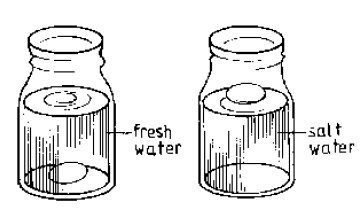
\includegraphics[width=0.45\textwidth]{./img/source/egg-float.png}
\end{center}

\begin{description*}
%\item[Subtopic:]{}
\item[Materials:]{2 fresh eggs, 2 containers (bottles cut in half), salt (less than half a cup)}
\item[Setup:]{Fill the two containers with water and place a fresh egg in each.}
\item[Procedure:]{Leave one as it is and add salt to the other. Add and mix salt until the egg floats in the saltwater container.}
%\item[Hazards:]{}
\item[Questions:]{Why does the egg float in saltwater but sink in fresh water?}
%\item[Observations:]{}
\item[Theory:]{Saltwater has a greater density than fresh water. A fresh egg has a density between fresh water and saltwater. Since an egg is denser than freshwater, it sinks. Since an egg is less dense than saltwater, it floats.}
\item[Applications:]{This is the same reason why it is easier to stay afloat when swimming in the ocean (saltwater) as opposed to a lake (fresh water).}
%\item[Notes:]{}
\end{description*}

\subsection{Floating Candle}

\begin{center}
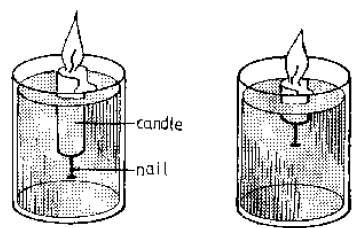
\includegraphics[width=0.45\textwidth]{./img/source/floating-candle.png}
\end{center}

\begin{description*}
%\item[Subtopic:]{}
\item[Materials:]{Candle, nail, container, water}
%\item[Setup:]{}
\item[Procedure:]{Put a nail into the bottom end of a candle so that the candle just floats with its top a bit above the surface of the water. Light the candle and watch as it burns up.}
%\item[Hazards:]{}
\item[Questions:]{Why does the candle continue to float even though it loses weight as it burns up?}
%\item[Observations:]{}
\item[Theory:]{The candle continues to float because its density remains less than that of the surrounding water.}
%\item[Applications:]{}
%\item[Notes:]{}
\end{description*}

\vfill

\subsection{Cartesian Diver}

\begin{center}
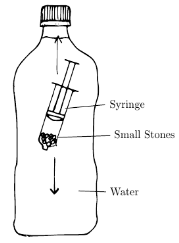
\includegraphics[width=0.3\textwidth]{./img/cartesian-diver.png}
\end{center}

\begin{description*}
%\item[Subtopic:]{}
\item[Materials:]{1.5 L plastic bottle, balloon, paper clips (large), water}
\item[Setup:]{Fill the bottle with water. Fix a large paper clip to the lip of a balloon. Making sure to keep all air out of the balloon, insert it into the bottle. It should just float at the top while remaining completely submerged. Adjust depending on type of balloon and paper clips.}
\item[Procedure:]{Screw the cap on the bottle and squeeze the middle of the bottle, then release.}
%\item[Hazards:]{}
%\item[Questions:]{}
\item[Observations:]{The balloon should begin to sink when you squeeze, but float again when you release.}
\item[Theory:]{While water is nearly incompressible, the balloon (and any small amount of air inside) is compressible. This means when you squeeze the bottle, the water remains unchanged, but the balloon is compressed, decreasing its volume and so increasing its density. Before squeezing, it was less dense than the water and so it floated. After squeezing, it becomes denser than the water and sinks.}
%\item[Applications:]{}
%\item[Notes:]{}
\end{description*}

\subsection{The Hydrometer}

\begin{center}
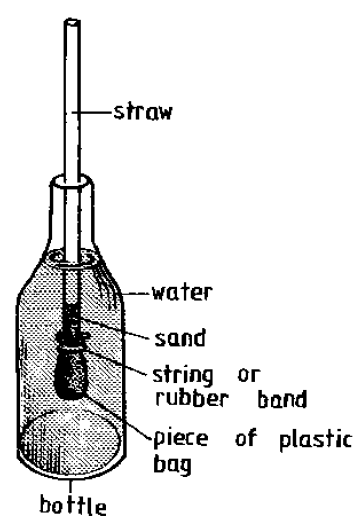
\includegraphics[width=0.3\textwidth]{./img/source/hydrometer.png}
\end{center}

\begin{description*}
%\item[Subtopic:]{}
\item[Materials:]{Bottle, straw, plastic bag, dry sand, rubber band/string, pen, ruler, water, kerosene, other liquids}
\item[Setup:]{Close one end of the straw with the plastic bag and secure it with the rubber band so that water cannot enter. Pour sand into the straw until it floats upright in the bottle of water without touching the bottom or leaning.}
\item[Procedure:]{Use a pen to mark the water level on the outside of the straw. Label it 1.0 (the density of water in g/cm$^3$). Place the straw upright in a container of kerosene. Mark the kerosene level on the straw as 0.8 (known density of kerosene). Remove and clean the straw, without getting any liquid inside. Use a ruler to complete the scale above 1.0 and below 0.8, beginning with 0.9 at the midpoint. Use the hydrometer to measure the densities of other liquids.}
%\item[Hazards:]{}
\item[Questions:]{Why do smaller numbers appear at the top of the hydrometer scale?}
%\item[Observations:]{}
\item[Theory:]{Liquids with a lower density allow the hydrometer to sink deeper, and thus the liquid reaches a higher point on the scale.}
%\item[Applications:]{}
%\item[Notes:]{}
\end{description*}


\end{multicols}

\pagebreak